\documentclass{article}
\usepackage[margin=0.75in]{geometry}
\usepackage{tikz}
\usetikzlibrary{positioning,arrows.meta,calc,shapes.geometric}
\usepackage{tcolorbox}
\usepackage{xcolor}

\newcommand{\benchmark}{ChessChain}

\begin{document}

\begin{figure}[t]
    \centering

    % Chess problem with explicit dependency graph
    \begin{tcolorbox}[
        title=\textbf{Chess: Minimax Search} \hfill {\small\colorbox{orange!20}{Easy} \quad 6 orderings},
        colframe=orange!70!black,
        colback=orange!3,
        boxrule=0.8pt,
        width=\textwidth
    ]
    \small

    \textbf{Dependency graph:}
    \begin{center}
    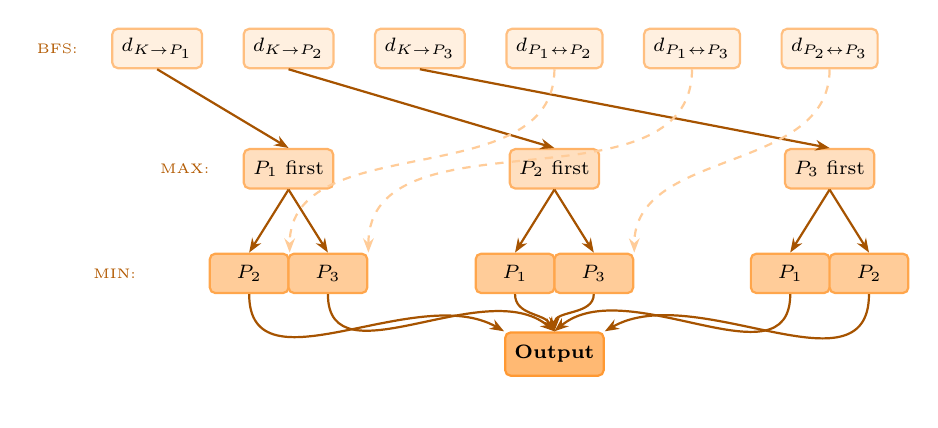
\begin{tikzpicture}[
        node distance=0.6cm and 0.8cm,
        every node/.style={font=\scriptsize},
        bfs/.style={draw, rounded corners=2pt, fill=orange!12, minimum width=0.9cm, minimum height=0.5cm, thick, draw=orange!50},
        maxnode/.style={draw, rounded corners=2pt, fill=orange!25, minimum width=1.0cm, minimum height=0.5cm, thick, draw=orange!60},
        minnode/.style={draw, rounded corners=2pt, fill=orange!40, minimum width=1.0cm, minimum height=0.5cm, thick, draw=orange!70},
        outputnode/.style={draw, rounded corners=2pt, fill=orange!55, minimum width=1.1cm, minimum height=0.55cm, thick, draw=orange!80, font=\scriptsize\bfseries},
        arrow/.style={-{Stealth[length=1.8mm]}, thick, orange!65!black}
    ]
        % Layer 0: BFS computations (shortest paths)
        \node[bfs] (bfs1) {$d_{K \to P_1}$};
        \node[bfs, right=0.5cm of bfs1] (bfs2) {$d_{K \to P_2}$};
        \node[bfs, right=0.5cm of bfs2] (bfs3) {$d_{K \to P_3}$};
        \node[bfs, right=0.5cm of bfs3] (bfs4) {$d_{P_1 \leftrightarrow P_2}$};
        \node[bfs, right=0.5cm of bfs4] (bfs5) {$d_{P_1 \leftrightarrow P_3}$};
        \node[bfs, right=0.5cm of bfs5] (bfs6) {$d_{P_2 \leftrightarrow P_3}$};

        % Label for BFS layer
        \node[font=\tiny, orange!70!black, anchor=east] at ([xshift=-0.3cm]bfs1.west) {BFS:};

        % Layer 1: Alice's first move (MAX) - which pawn to capture first
        \node[maxnode, below=1.0cm of bfs2] (max1) {$P_1$ first};
        \node[maxnode, below=1.0cm of bfs4] (max2) {$P_2$ first};
        \node[maxnode, below=1.0cm of bfs6] (max3) {$P_3$ first};

        % Label for MAX layer
        \node[font=\tiny, orange!70!black, anchor=east] at ([xshift=-0.3cm]max1.west) {MAX:};

        % Layer 2: Bob's response (MIN) - which pawn next
        \node[minnode, below=0.8cm of max1, xshift=-0.5cm] (min1a) {$P_2$};
        \node[minnode, below=0.8cm of max1, xshift=0.5cm] (min1b) {$P_3$};
        \node[minnode, below=0.8cm of max2, xshift=-0.5cm] (min2a) {$P_1$};
        \node[minnode, below=0.8cm of max2, xshift=0.5cm] (min2b) {$P_3$};
        \node[minnode, below=0.8cm of max3, xshift=-0.5cm] (min3a) {$P_1$};
        \node[minnode, below=0.8cm of max3, xshift=0.5cm] (min3b) {$P_2$};

        % Label for MIN layer
        \node[font=\tiny, orange!70!black, anchor=east] at ([xshift=-0.8cm]min1a.west) {MIN:};

        % Layer 3: Final capture (implicit - last remaining pawn)

        % Layer 4: Output - minimax result
        \node[outputnode, below=1.0cm of max2, yshift=-0.8cm] (out) {\textbf{Output}};

        % Arrows from BFS to MAX nodes
        \draw[arrow] (bfs1.south) -- (max1.north);
        \draw[arrow] (bfs2.south) -- (max2.north);
        \draw[arrow] (bfs3.south) -- (max3.north);

        % Arrows from MAX to MIN
        \draw[arrow] (max1.south) -- (min1a.north);
        \draw[arrow] (max1.south) -- (min1b.north);
        \draw[arrow] (max2.south) -- (min2a.north);
        \draw[arrow] (max2.south) -- (min2b.north);
        \draw[arrow] (max3.south) -- (min3a.north);
        \draw[arrow] (max3.south) -- (min3b.north);

        % Arrows from BFS to MIN (for transition distances)
        \draw[arrow, dashed, orange!40] (bfs4.south) to[out=-90, in=90] (min1a.north east);
        \draw[arrow, dashed, orange!40] (bfs5.south) to[out=-90, in=90] (min1b.north east);
        \draw[arrow, dashed, orange!40] (bfs6.south) to[out=-90, in=90] (min2b.north east);

        % Arrows from MIN to Output (minimax backprop)
        \draw[arrow] (min1a.south) to[out=-90, in=150] (out.north west);
        \draw[arrow] (min1b.south) to[out=-90, in=140] (out.north);
        \draw[arrow] (min2a.south) to[out=-90, in=120] (out.north);
        \draw[arrow] (min2b.south) to[out=-90, in=90] (out.north);
        \draw[arrow] (min3a.south) to[out=-90, in=40] (out.north);
        \draw[arrow] (min3b.south) to[out=-90, in=30] (out.north east);

    \end{tikzpicture}
    \end{center}

    \vspace{-0.1cm}
    \begin{tabular}{@{}p{0.48\textwidth}p{0.48\textwidth}@{}}
    \textit{Step 1:} BFS computes shortest knight paths between all positions ($K$, $P_1$, $P_2$, $P_3$). &
    \textit{Step 2:} Minimax over $3! = 6$ capture orderings with Alice (MAX) and Bob (MIN) alternating. \\
    \end{tabular}

    \vspace{0.2cm}
    \hfill \textbf{Answer:} [Redacted]
    \end{tcolorbox}

    \caption{\textbf{Chess dependency graph:} \colorbox{orange!12}{BFS nodes} compute shortest paths, \colorbox{orange!25}{MAX nodes} represent Alice's choices (maximize total moves), \colorbox{orange!40}{MIN nodes} represent Bob's choices (minimize). Dashed arrows show distance lookups; solid arrows show game tree structure.}
\end{figure}

\end{document}
